%\documentclass{amsart}

\documentclass{article}
\usepackage[letterpaper,hmargin=15mm,vmargin=20mm]{geometry}
\usepackage[nosetup, colorlinks]{tony}
\usepackage{graphicx}

\usepackage{amsmath,amssymb}
\usepackage{mathpazo}
\usepackage{multicol}
\usepackage{diagbox}

\usepackage{caption}% http://ctan.org/pkg/caption
\usepackage[labelformat=simple]{subcaption}% http://ctan.org/pkg/subcaption
\newcommand{\pic}[1]{\rule{#1}{#1}}% Fake picture of size #1 x #1
\renewcommand\thesubfigure{(\alph{subfigure})}% Allow sub-figure reference to be correctly printed

\usepackage{xcolor}
%\usepackage[printwatermark]{xwatermark}
%\newwatermark*[allpages,color=gray!50,angle=45,scale=3,xpos=0,ypos=0]{DRAFT}

\DeclareMathOperator{\sgn}{sgn}
\DeclareMathOperator{\NLL}{NLL}
\newcommand{\sind}[1]{^{(#1)}}

\title{6.867: Problem Set 2}
\date{October 25, 2016}

\begin{document}
\maketitle

\begin{multicols}{2}

% % % % % % % % % %
%    PROBLEM 1
% % % % % % % % % %

\section{Logistic Regression}
\label{sec:lr}

We implemented logistic regression with $L_2$ regularization.
Recall that the objective function for $L_2$ regularization takes the form
\begin{equation}
    E_{LR}(w, w_0) = \NLL(w, w_0) + \lambda ||w||_2^2
\end{equation}
where NLL is the logistic loss
\begin{equation}
    \text{NLL}(w, w_0) = \sum_i{\log(1+\exp(-y^{(i)}(w\cdot x^{(i)}+w_0)))}
\end{equation}
and the $y\sind{i}$ are labels $\pm 1$.
We minimized the objective function by gradient descent;
note that the gradient of $E_{LR}$ with respect to $w$ is
\begin{equation}
    \f{d E_{LR}}{dw} = \sum_{i=1}^n\lt(s(w\cdot x^{(i)})-y^{(i)}\rt)x^{(i)} - 2\lambda w
\end{equation}
where $s(x) = 1/(1+e^{-x})$ is the sigmoid function.

We tested our implementation against four artificial datasets,
the first three with 400 training samples,
200 validation samples,
and 200 testing samples, and fourth with 400 training, validation, and testing samples.
The data consisted of two-dimensional vectors $x\sind{i}$ labeled by $y\sind{i} = \pm1$.

As gradient descent progressed,
we observed that $||w||$ decreased, eventually converging. When we set $\lambda = 1$, 
$||w||$ was penalized, converging to a slightly smaller magnitude than when $\lambda = 0$.
However, this effect was subtle.
%When we set $\lambda = 1$, $||w||$ is penalized,
%we see that there is less fluctuation in $||w||$ (Figure~\ref{fig:weight-regularization}).
%The exact shift in $||w||$, however,
%was quite sensitive to changes in initial guess.
% TODO ^^ be more clear

%  (Figure~\ref{fig:weight-regularization}). 
%\begin{figure*}
%   \centering
%   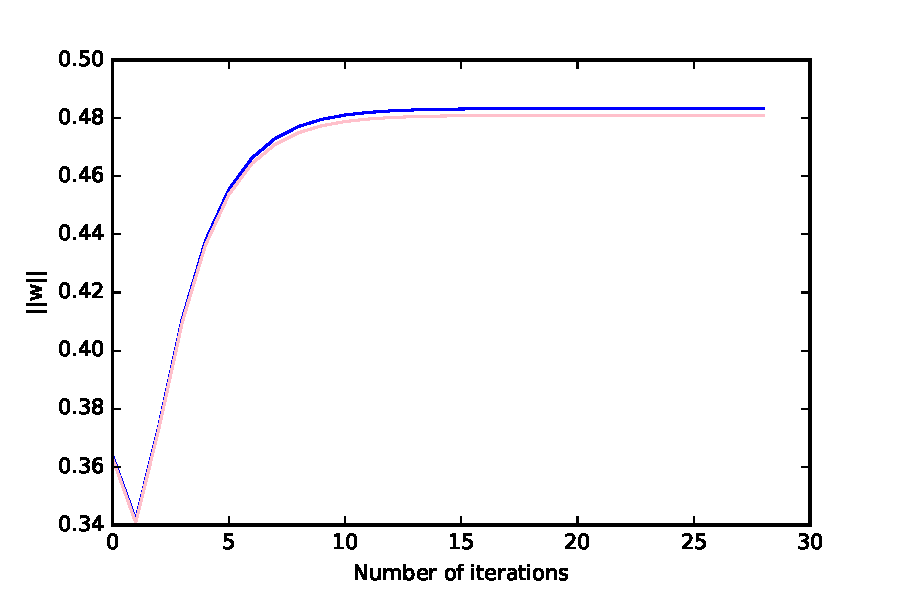
\includegraphics[width=3in]{img/1-1-weights.pdf}
%   \caption{Effects of regularization on weight vector. I promise I'll replace this.}
%   % TODO please replace
%   \label{fig:weight-regularization}
%\end{figure*}

\begin{figure*}
   \centering
   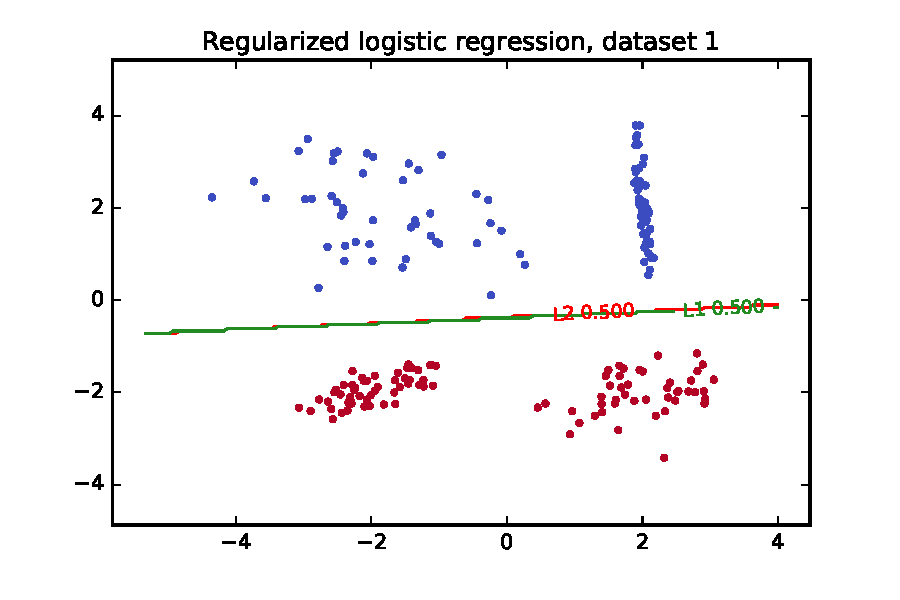
\includegraphics[width=3in]{img/1-3-1.pdf}
   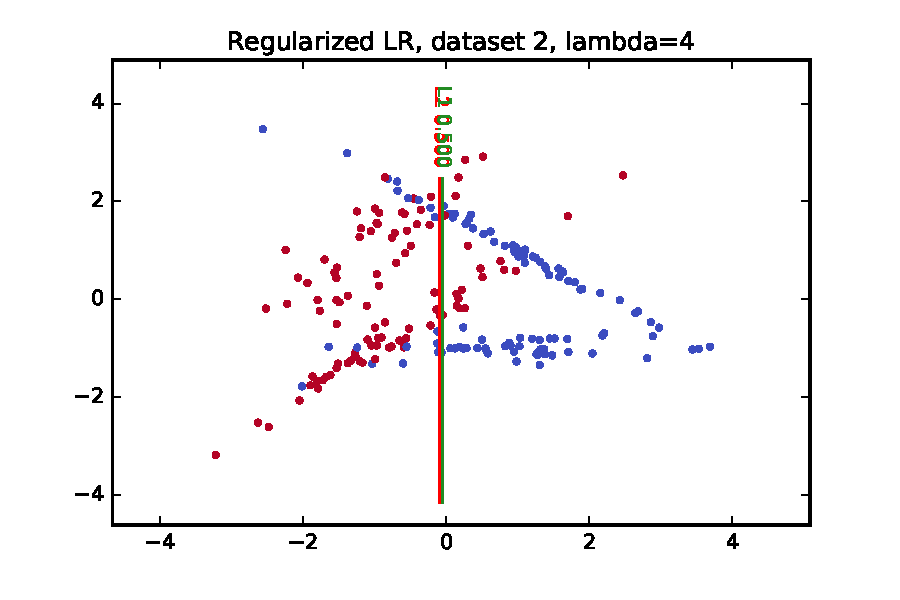
\includegraphics[width=3in]{img/1-3-2.pdf}
   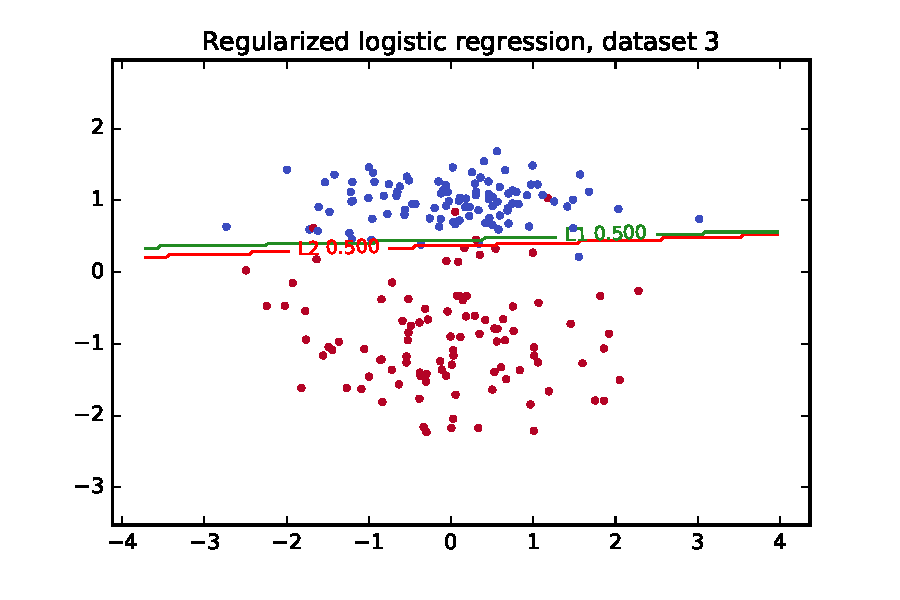
\includegraphics[width=3in]{img/1-3-3.pdf}
   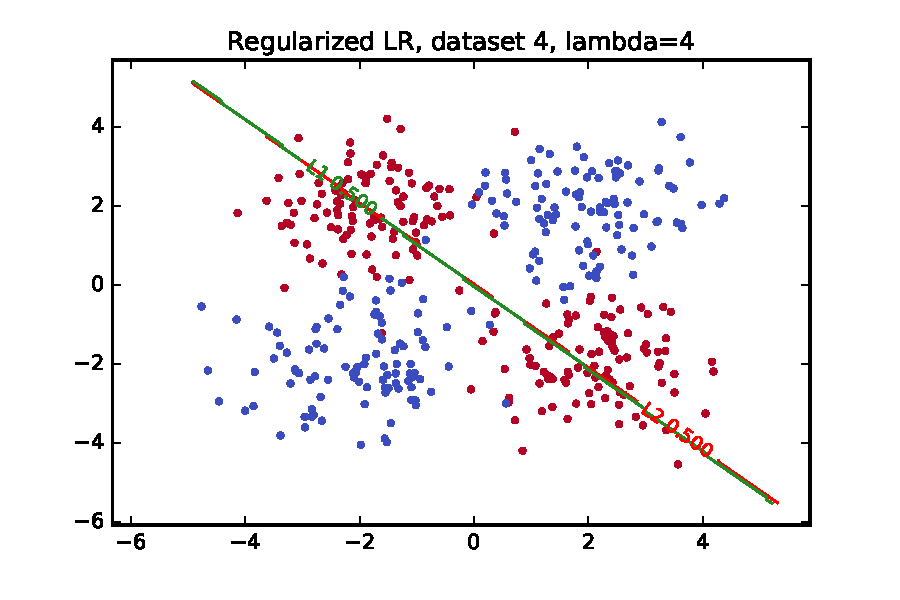
\includegraphics[width=3in]{img/1-3-4.pdf}
   \caption{Decision boundaries from $L_2$ and $L_1$ normalization. The red line is the $L_2$ boundary; the green, $L_1$. Datasets 1 and 3 are more or less separable, while datasets 2 and 4 are adverse examples. Classification accuracy for $L_2$ and $L_1$ were respectively, in order of dataset, 1.0 and 0.995; 0.81 and 0.81; 0.97 and 0.975; 0.4975 and 0.5.}
   % TODO please replace
   \label{fig:1-3-boundaries}
\end{figure*}

\subsection{$L_1$ and $L_2$ Regularization}
We compared the effects of $L_1$ and $L_2$ regularization.
Recall that the objective function with $L_1$ regularization is
\begin{equation}
    E_{LR}(w, w_0) = \NLL(w, w_0) + \lambda ||w||_1
\end{equation}
where $||w||_1 = \sum_{i=1}^n{|w_i|}$. 
While $L_2$ regularization maintained small values throughout $w$, $L_1$ allowed for sparse $w$, especially when $\lambda$ increased. $L_1$ also tended to be less stable, causing more fluctuations in $w$ across different $\lambda$. At high $\lambda$ (e.g. $\lambda = 8$), the sparser $L_1$ weights led to higher classification error than the $L_2$ weights. However, both regularization schemes produced similar decision boundaries, as drawn in Figure \ref{fig:1-3-boundaries}.
%For small $\lambda$,
%$L_2$ regularization resulted in smaller weights
%than $L_1$ regularization, since the magnitude of $w$ is penalized more.

We selected the optimal hyperparameters for each dataset
by rate of misclassification on the validation set.
Some datasets did not have a unique optimal parameter.
For these, we arbitrarily selected one.
We evaluated these optimal models' performance on our test sets;
we present our results below.
\begin{center}
\begin{tabular}{|c||c|c|c|}
\hline
dataset & $\lambda$	& regularization		 & accuracy \\\hline
        1	&  1.0 & $L_2$ & 1.0\\
        2	& 4 & $L_2$ & 0.81 \\
        3	& 4 & $L_1$ & 0.975 \\
        4	& 1.0 & $L_1$ & 0.5 \\\hline
\end{tabular}
\end{center}
%
%\begin{table*}
%    \caption{Classification performance on testing datasets.}
%    % TODO please fix this
%    \centering
%    \begin{tabular}{|c||c|c|c|}
%        \hline
%        dataset & $\lambda$	& regularization		 & accuracy \\\hline
%        1	&  1.0 & L2 & 1.0\\
%        2	& 4 & L1 & 0.81 \\
%        3	& 4 & L1 & 0.975 \\
%        4	& 1.0 & L2 & 0.5 \\\hline
%    \end{tabular}
%    \label{table:1-3-optimal}
%\end{table*}

% % % % % % % % % %
%    PROBLEM 2
% % % % % % % % % %

\section{Support Vector Machines (SVMs)}
\label{sec:svm}

\subsection{Dual Soft-SVM}

We implemented the dual form of soft-SVM
with third-party convex optimization software.
Recall that the soft-SVM dual optimization problem takes the form
\begin{equation}
    \label{eq:soft-svm-dual}
    \begin{array}{ll@{}ll}
        \text{maximize}  &\displaystyle -\f{1}{2}\sum_{i,j} \alpha_i \alpha_j y\sind{i} y\sind{j} \angb{x\sind{i}, x\sind{j}}
        +
        \sum_i \alpha_i \\
        \text{subject to}& 0 \le \alpha_i \le C\\
        & \displaystyle\sum_{i=1}^n \alpha_i y\sind{i} = 0
    \end{array}
\end{equation}
for training data $x\sind{i}$
labeled by $y\sind i = \pm 1$.
Hyperparameter~$C$ controls the amount of slack we permit.
Given a new data point $x$,
we predict its label $y$ as
\begin{equation}
    \label{eq:soft-svm-predict}
    y = \sgn\lt(\sum_i \alpha^*_i y\sind{i} \angb{x\sind{i}, x}\rt) \equiv \sgn(t(x))
\end{equation}
where $\alpha^*_i$ is the optimal value of $\alpha_i$
from Equation~\ref{eq:soft-svm-dual}.

For instance, on a toy dataset with positive examples
$(2, 2), (2, 3)$ and negative examples $(0, -1), (-3, -2)$,
our optimization problem takes the form
\begin{equation}
    \label{eq:soft-svm-dual-concrete}
    \begin{array}{ll@{}ll}
        \text{maximize}  &\displaystyle -\f{1}{2}\alpha^T
        \left[
            \begin{array}{cccc}
                8 & 10 & 2 & 10 \\
                10 & 13 & 3 & 12 \\
                2 & 3 & 1 & 2 \\
                10 & 12 & 2 & 13
            \end{array}
        \right]
        \alpha
        +
        \sum_{i=1}^4 \alpha_i \\
        \text{subject to}& 0 \le \alpha_i \le C\\
        & \alpha_1 + \alpha_2 = \alpha_3 + \alpha_4
    \end{array}
\end{equation}
Upon inspection,
it is clear that for large $C$
(i.e. in the hard-SVM limit),
the support vectors are $(2,2)$ and $(0,-1)$.


We tested our soft-SVM implementation
on the same four 2D datasets from the previous section.
Setting regularization parameter $C=1$,
we get the following support vector counts
and misclassification rates on validation data:

\begin{center}
\begin{tabular}{|c|c|c|}
\hline
Dataset & Support vectors & Misclassification \\\hline
1 & 4/400 & 0/200 \\
2 & 174/400 & 36/200 \\
3 & 33/400 & 6/200 \\
4 & 392/400 & 122/400\\\hline
\end{tabular}
\end{center}

Our model clearly performs better in datasets 1 and 3.
Indeed, these datasets are linearly separable (or very nearly so),
as is apparent from Figure~\ref{fig:2-3-model-selection},
where the test data from each dataset are plotted.
Observe also that the number of support vectors
generally tracks the misclassification rate.

In the next section, we will kernelize our SVM routine
to handle nonlinearities in our data
(for instance, the XOR data in dataset 4 is roughly separable, but only nonlinearly).



\subsection{Kernelization}
\label{subsec:kernelization}

It is often useful to map our raw data
with some nonlinear feature map $\phi$
into a higher dimensional feature space.
However, it is often infeasible to compute and store in memory
all the values $\phi(x\sind{i})$.

Therefore, we recall the ``kernel trick": the insight that
because Equation~\ref{eq:soft-svm-dual} and \ref{eq:soft-svm-predict}
only refer to values $\phi(x\sind{i})$ inside inner products
with other $\phi(x\sind{j})$,
we only need the kernel function
\begin{equation}
    k(x, x') = \angb{\phi\lt(x\rt), \phi\lt(x'\rt)},
\end{equation}
which is usually much easier to compute than the feature map $\phi$.

By replacing the inner products in
Equations~\ref{eq:soft-svm-dual} and \ref{eq:soft-svm-predict}
with the corresponding kernels,
we arrive at the kernelized soft-SVM optimization problem.
Thus, we kernelized our SVM routine
and tested it with a linear kernel
\begin{equation}
    k(x, x') = x\cdot x'
\end{equation}
and with Gaussian RBF kernels
\begin{equation}\label{eq:2-2-gaussian-rbf}
    k(x, x') = \exp\lt(-\f{|x - x'|^2}{2\sigma^2}\rt)
\end{equation}
with bandwidths~$\sigma=0.25,0.5,1.0,2.0$ on the same four datasets as before.
We took
\[
    C \in \{0.01, 0.1, 1, 10, 100\}.
\]

In particular, we performed model selection as follows:
within both the family of linear SVMs (parametrized by $C$)
and the family of RBF SVMs (parametrized by $C$ and $\sigma$).
we took the hyperparameters that produced the best model by validation error
(using misclassification as our error metric).
Finally, we took the best of the best two models (again by validation error).
We show these best models on test data in Figure~\ref{fig:2-3-model-selection}
along with the corresponding test errors.

\begin{figure*}[t]
   \centering
   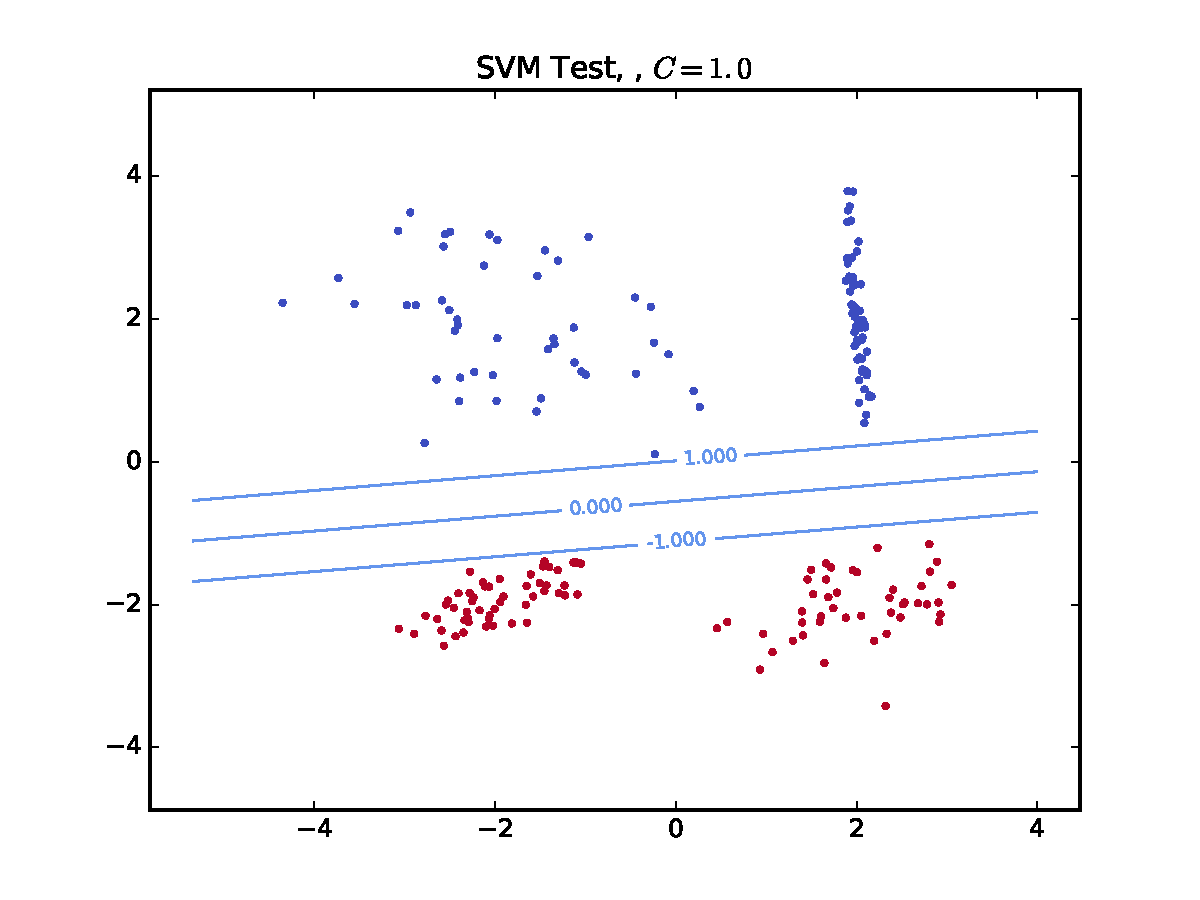
\includegraphics[width=3in]{img/p2-3-d1-c001/test.pdf}
   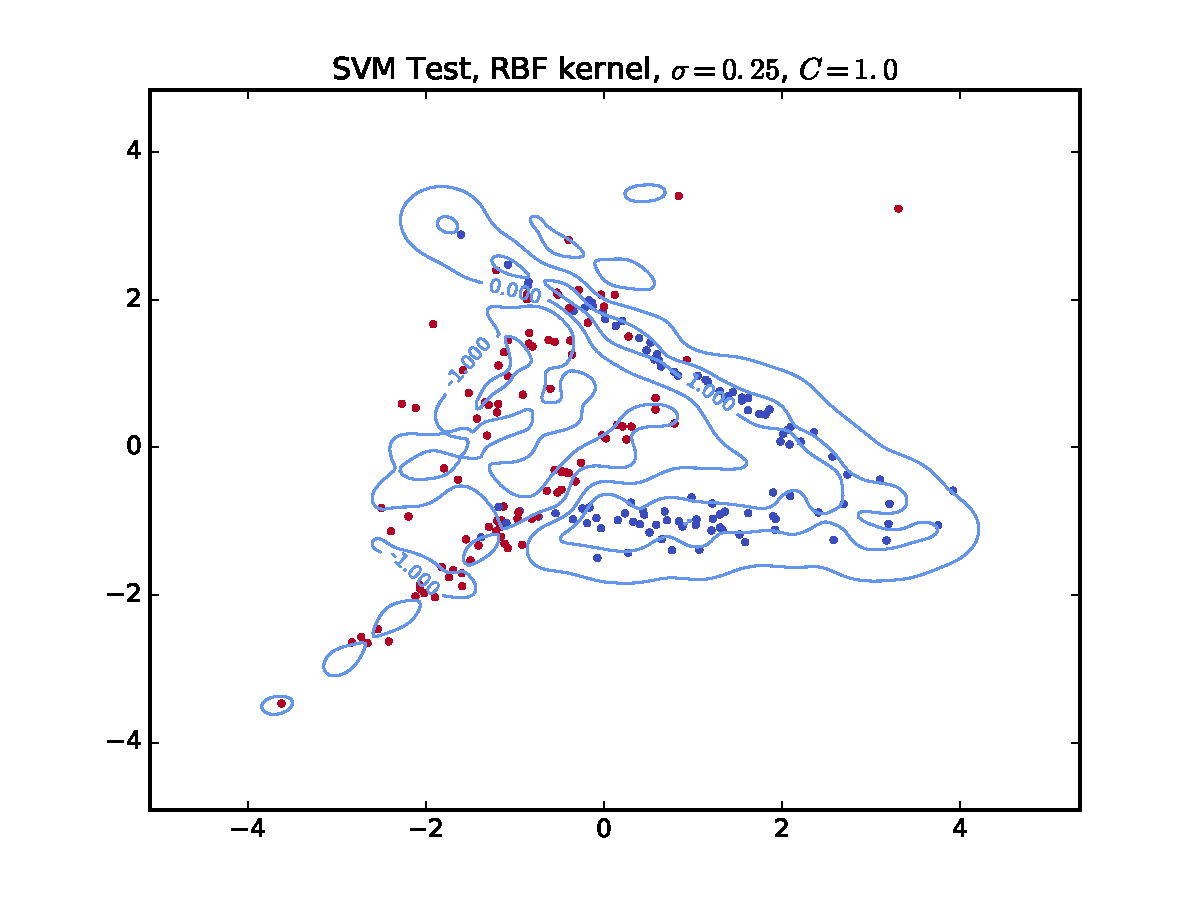
\includegraphics[width=3in]{img/p2-3-d2-c1-rbf025/test.pdf}
   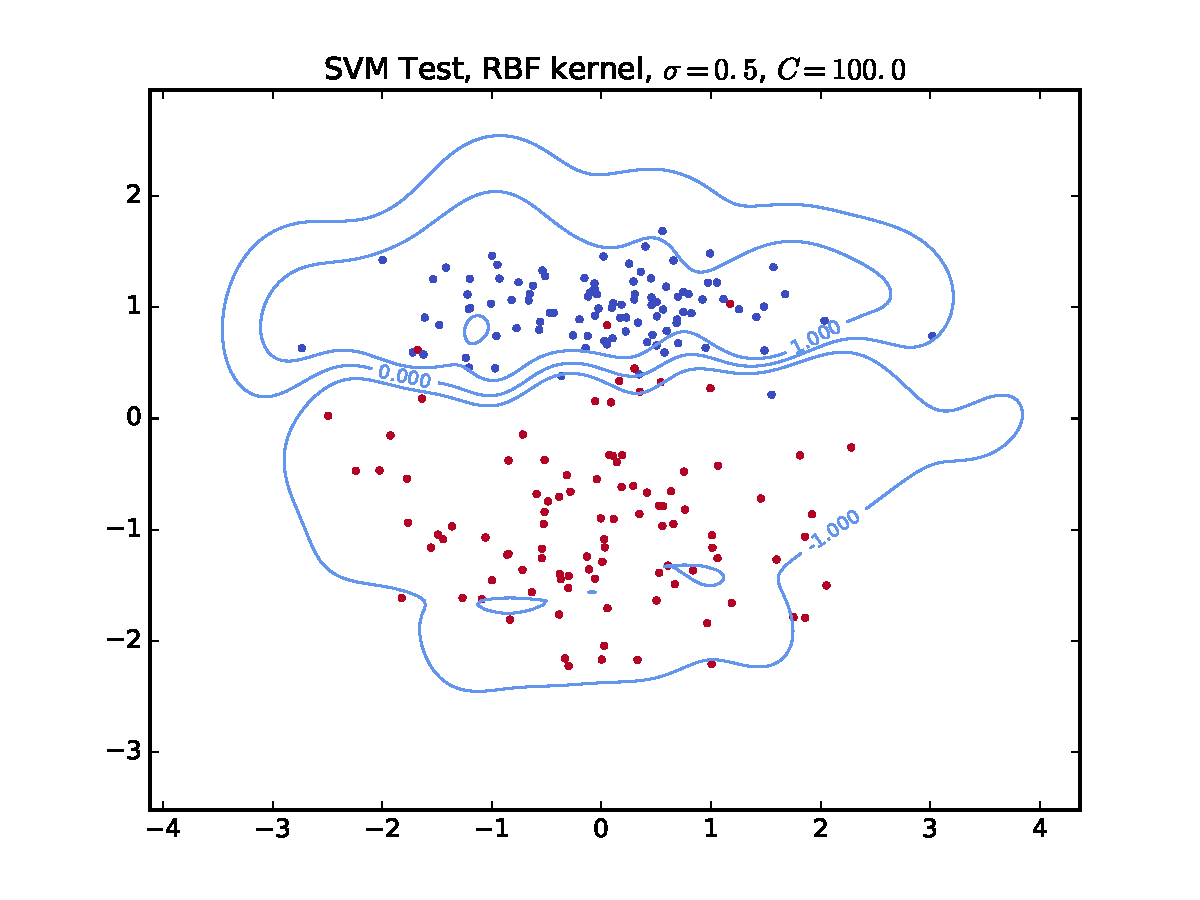
\includegraphics[width=3in]{img/p2-3-d3-c100-rbf025/test.pdf}
   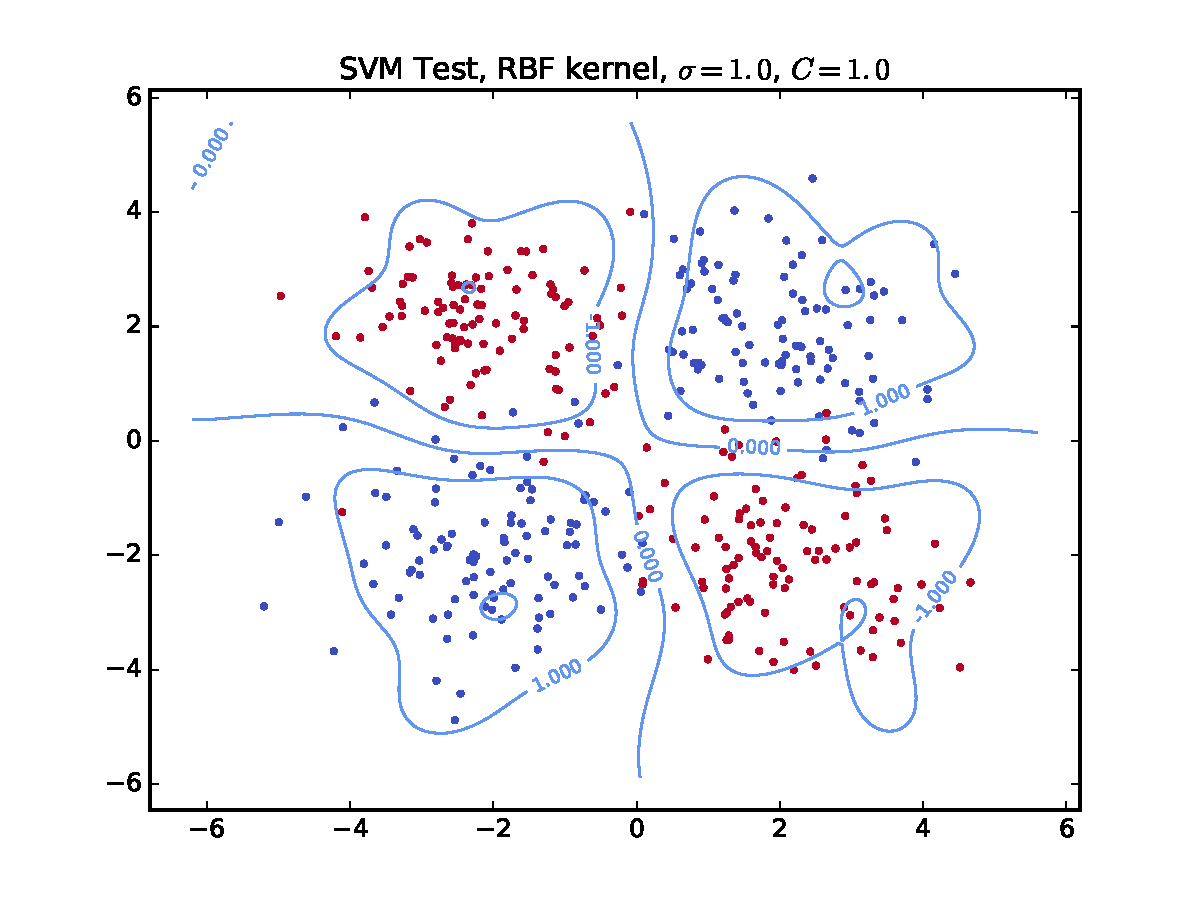
\includegraphics[width=3in]{img/p2-3-d4-c1-rbf10/test.pdf}
   \caption{Decision boundaries (with contours $t = \pm1$)
   on test data for best models produced by model selection.
   For each dataset, our best model had a misclassification rate of 0, 6, 3.5, 4.25\%, respectively.}
   \label{fig:2-3-model-selection}
\end{figure*}

In the linearly separable case, with a linear kernel,
we found that increasing $C$ led to tighter margins and fewer support vectors.
The model made no misclassifications on the validation data for $C$ in the range we tested.

Gaussian kernels worked well when we chose bandwidth~$\sigma$
commensurate to the size of the spatial features of the dataset.
Excessively small $\sigma$ created decision boundaries that overfit to training data.
On the other hand, models with $\sigma$ too large were unable to discern tight structure.
We illustrate these findings in Figure~\ref{fig:2-3-gaussian-rbf}.

In general,
Gaussian kernel SVMs have lower bias,
but introduce greater variance,
since using RBF kernels is equivalent to
mapping the raw data into an infinite-dimensional feature space.
This lower bias is manifested
in the larger number of support vectors
and in the tighter shapes of the decision boundaries.

\begin{figure*}[t]
   \centering
   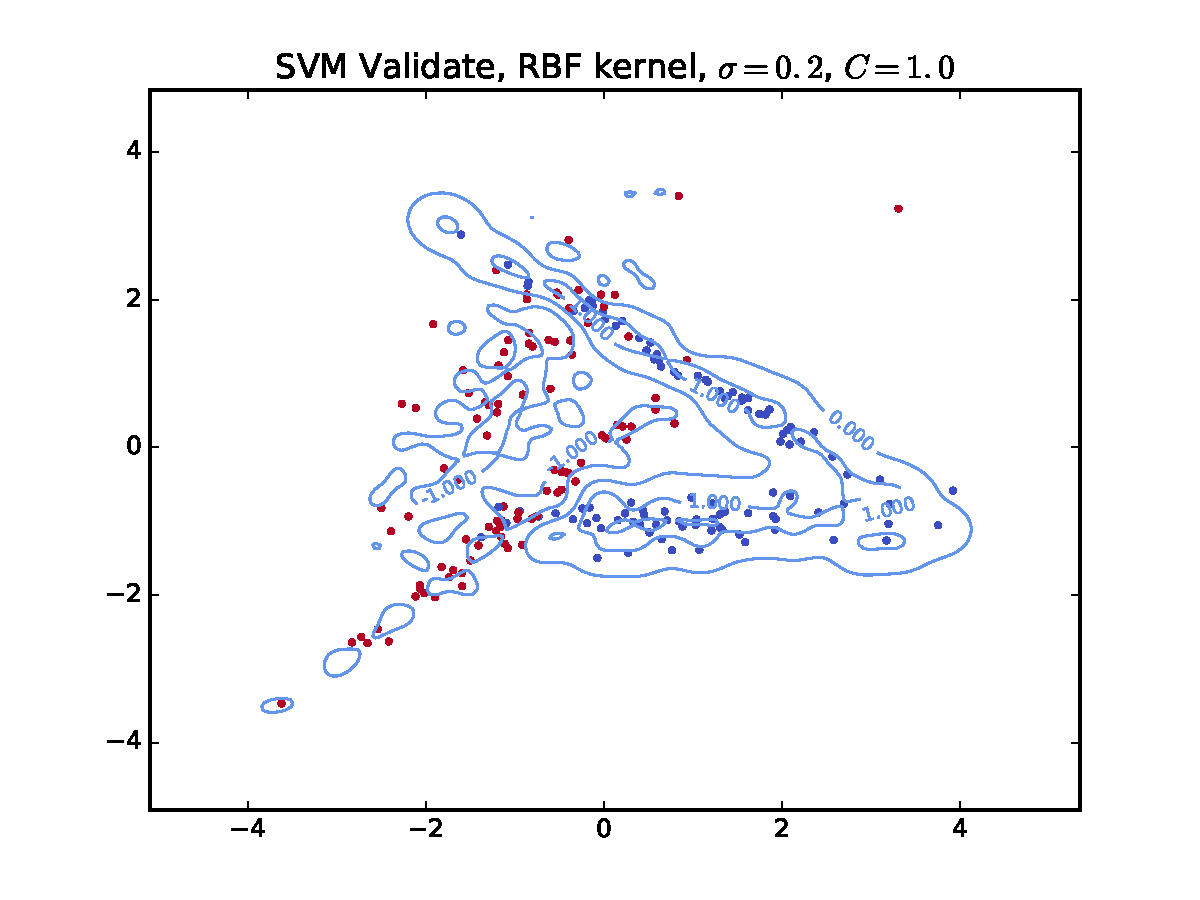
\includegraphics[width=2.4in]{img/p2-3-d2-c1-rbf02/validate.pdf}
   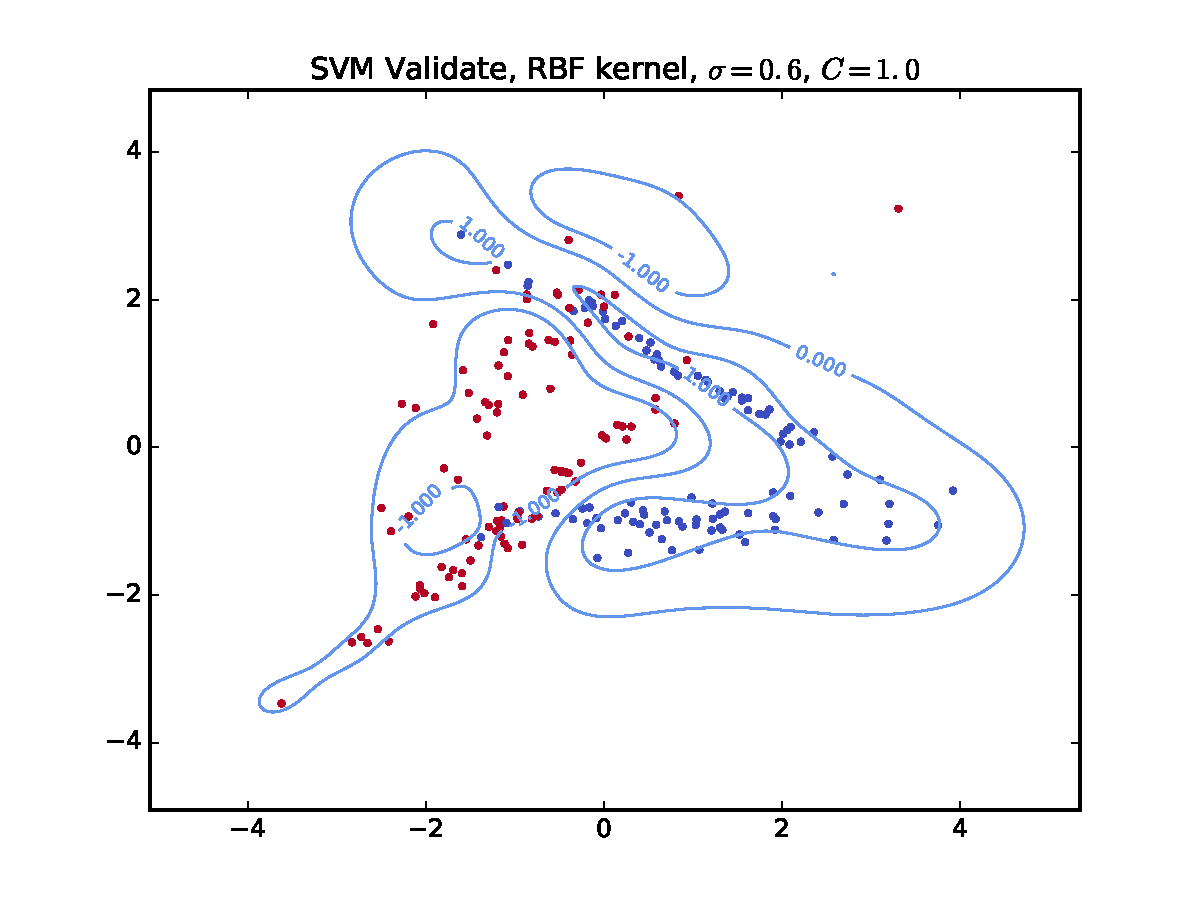
\includegraphics[width=2.4in]{img/p2-3-d2-c1-rbf06/validate.pdf}
   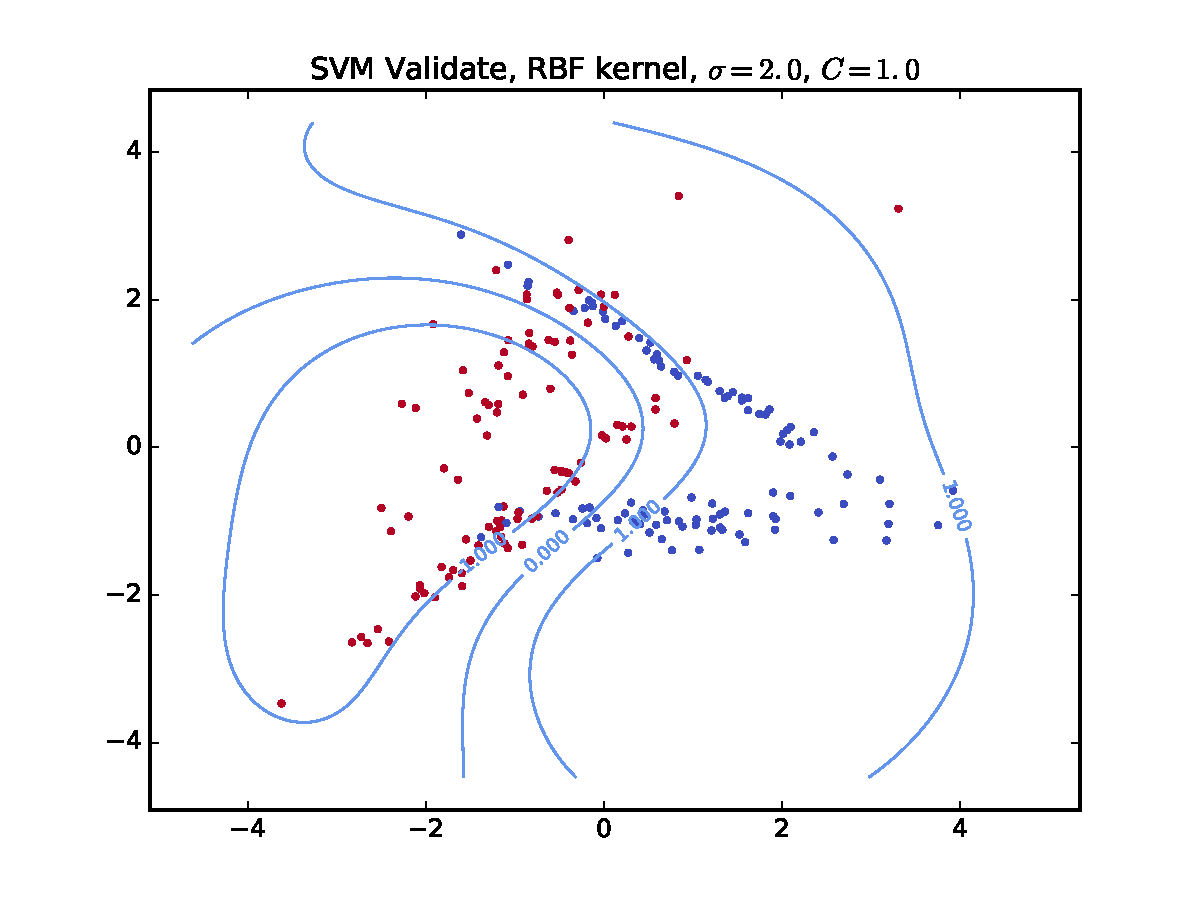
\includegraphics[width=2.4in]{img/p2-3-d2-c1-rbf20/validate.pdf}
   \caption{SVM decision boundaries (with contours $t = \pm1$) on validation data
   for dataset 2, with $C = 1$ and Gaussian RBF kernels
   with bandwidths $\sigma=0.2,0.6,2.0$, in that order.}
   \label{fig:2-3-gaussian-rbf}
\end{figure*}

We make some observations about hyperparameter~$C$.
From Equation~\ref{eq:soft-svm-dual},
larger $C$ corresponds to less tolerance for slack.
For small $C$, the model favors
maximizing the margin at the expense of slack,
so we expect increasing $C$ shrinks the geometric margin,
as our experiments confirm.

Consequently, there are fewer support vectors with large $C$:
the margin becomes tighter,
and the model grows increasingly averse to margin errors,
which make up the bulk of the support vectors for small $C$.

The size of the margin
is not a good metric for choosing $C$,
as can make the margin arbitrarily large
by taking $C \to 0$
(indeed, $C = 0$ allows arbitrary amounts of slack
with no penalty on the objective function).
We'd instead like a metric that evaluates
the performance of a given $C$
on unseen data.

One such metric is the hinge loss incurred
by our classifier on a validation dataset:
\begin{equation}
    \sum_{i} \max\lt(0, 1 - y\sind{i} t\lt(x\sind{i}\rt)\rt)
\end{equation}
where $t$ is the prediction function in Equation~\ref{eq:soft-svm-predict}
and where the sum is taken over all validation data.
We could also use classification error on the validation set.


% % % % % % % % % %
%    PROBLEM 3
% % % % % % % % % %

\section{SVMs with Pegasos}

While generally effective, convenient, and efficient,
SVMs become unwieldy to solve as they become large.
Instead, we may consider solving the following soft-SVM
using the Pegasos algorithm
(primal estimated sub-gradient solver for SVM):
\begin{equation}
   \min_w \lt( \f{\lambda}{2}||w||^2 + \f{1}{n}\sum_{i=1}^n{\max\{0,1-y_i(w^Tx_i)\}} \rt)
\end{equation}
This problem is equivalent to C-SVM for $C= \f{1}{n\lambda}$.
Given a regularization parameter $\lambda$
and some maximum number of ``epochs,''
Pegasos stochastically updates our weight vector $w$ as follows.
\begin{enumerate}
\item Initialize $t$ and $w_0$ to 0.
\item At each iteration, increment $t$ and set a decaying step size $\eta_t = 1/(t\lambda)$.
\item If $y_i(w_t^Tx_i)<1$, then $w_{t+1}\leftarrow(1-\eta_t\lambda)w_t+\eta_ty_ix_i$. Else,  $w_{t+1}\leftarrow(1-\eta_t\lambda)w_t$.
\item Repeat until $t$ reaches the maximum number of epochs.
\end{enumerate}
We implemented the Pegasos algorithm and included a bias term $w_0$
that we did not penalize by regularization.
(We simply update $w_0$ as $w_0 = w_0 + \eta_t y_i$.)

Now recall that we define the margin as $||w||\inv$.
The regularization constant $\lambda$ limits the magnitude of $w$,
so as we increase $\lambda$, the margin grows.
We show this effect empirically in Figure~\ref{fig:3-2-margins} for a sample dataset.

% TODO

\begin{figure*}[t]
   \centering
	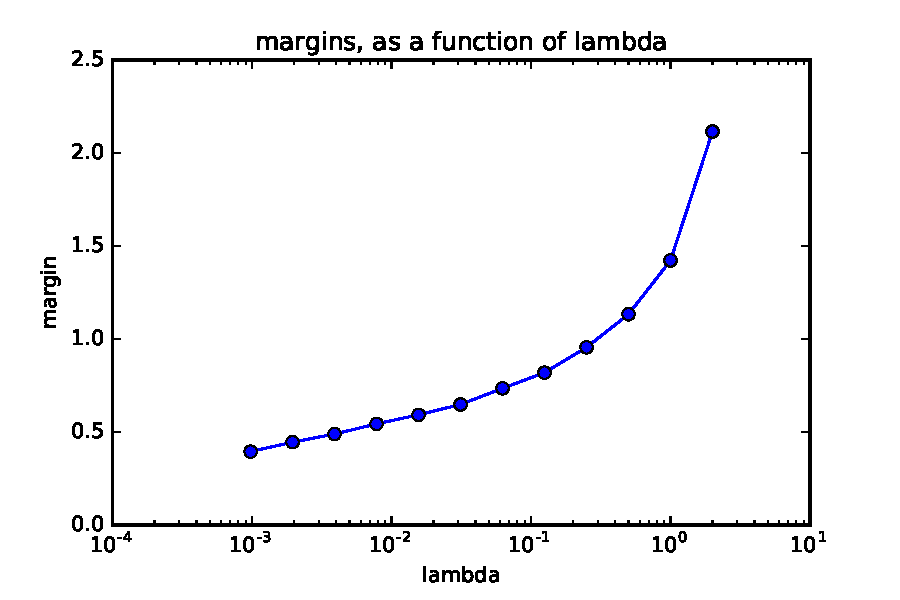
\includegraphics[width=3in]{img/3-2-margins.pdf}
   \caption{Effect of changing $\lambda$ on margins}
   \label{fig:3-2-margins}
\end{figure*}

\subsection{Kernelized Pegasos}
\label{subsec:kernel-peg}

We can extend the Pegasos algorithm
to solve the following kernelized soft-SVM problem:
\begin{equation}
   \min_w{\f{\lambda}{2}||w||^2} + \f{1}{n}\sum_{i=1}^n{\max\{0,1-y_i(w^T\phi(x_i))\}}
\end{equation}
where we map $x$ to some transformation $\phi(x)$ (above we simply took an identity $\phi$.)
The following kernelized Pegasos algorithm takes in a Gram matrix, 
where entry $k_{i,j} = K(x^{(i)},x^{(j)}) = \phi(x^{(i)})\cdot\phi(x^{(j)})$.
\begin{enumerate}
\item Initialize $t$ and $\alpha_{t=0}$ to 0.
\item At each iteration, increment $t$ and set a decaying step size $\eta_t = 1/(t\lambda)$.
\item If $y_i(\sum_j{\alpha_jK(x_j,x_i)})<1$, then $\alpha_{i}\leftarrow(1-\eta_t\lambda)\alpha_i+\eta_ty_i$. Else,  $\alpha_{i}\leftarrow(1-\eta_t\lambda)\alpha_i$.
\item Repeat until $t$ reaches the maximum number of epochs.
\end{enumerate}
Note that the primary difference between the kernelized Pegasos and the original version is that in place of a $d$ dimensional $w_t$, we now store $\alpha_i$ for each training instance; and in place of $x_i$, we apply some transformation $\phi(x_i)$.

The vector $\alpha$ may be sparse, with non-zero entries for support vectors (similar to the dual-SVM solution). Given optimal support vector values $\alpha_i$ and a new datapoint $x$, we predict its label $y$ as
\begin{equation}
    y = \sgn\left(\sum_i{a_i K(x,x^{(i)})}\right)
\end{equation}

We implemented the kernelized Pegasos algorithm with a Gaussian RBF kernel
(as in Equation \ref{eq:2-2-gaussian-rbf}), given fixed $\lambda = 0.02$, varying bandwidths $\gamma = \{2^{-2},\dots,2^2\}$, and maximum number of epochs = 10000.
We observed that smaller values of $\gamma$ resulted in fewer support vectors.

\begin{center}
\begin{tabular}{|c||c|c|c|c|c|}
\hline
$\gamma$ & $2^{-2}$ & $2^{-1}$ & 1 & 2 & 4\\ \hline
SV & 1/400 & 1/400 & 2/400 & 45/400 & 100/400 \\ \hline
\end{tabular}
\end{center}
Thus, the decision boundary becomes tighter as we decrease $\gamma$.

% % % % % % % % % %
%    PROBLEM 4
% % % % % % % % % %

\section{MNIST Digit Recognition}

We apply these various classifiers to the MNIST dataset
of $28\times 28$ grayscale images of handwritten digits:
each of the $28^2$ features corresponding to an image takes on an integer value in $[0, 255]$,
representing the grayscale luminescence of each pixel.

We optionally normalized input pixel features to the range $[-1, 1]$,
so that an input vector $x$ is mapped to $\f{2x}{255}-1$,
with all operations applied componentwise.

For all our following experiments,
we chose pairs of disjoint subsets of digits
to use as our positive and negative classes for binary classification.
Our training sets contained 250 samples of each digit in either of the two classes,
and our validation and test sets each contained 150 samples of each digit.

\subsection{Linear Models}

We begin by exploring the efficacy of our linear models on MNIST.
In particular, we will compare logistic regression from section~\ref{sec:lr}
with the linear SVM classifier from section~\ref{sec:svm}.
We experimented with the following binary classification problems;
the results of our experiments
(optimal hyperparameters and their test set misclassification rates)
are listed next to them.
\begin{center}
\begin{tabular}{|c|c||c|c||c|c|c|}
\hline
+ & - & $\lambda$ & LR error & $C$ & SVM error \\\hline
1 & 7 & 0.5 & 3/300 & 0.01 & 4/300 \\
3 & 5 & 0.5 & 18/300 & 0.01 & 16/300 \\
4 & 9 & 0.5 & 12/300 & 0.01 & 17/300\\
even & odd & 0.5 & 225/1500 & 0.01 & 245/1500\\\hline
\end{tabular}
\end{center}

Note that we used unnormalized data for both.
Normalization did not significantly affect test set accuracy
for either model.

We also manually inspected some of the classification errors.
These images were generally very ambiguous
(for example, a 4 that looks very much like a 9),
explaining their misclassification.


% TODO STUFF


\subsection{SVMs with RBF kernels}

Next, we introduced nonlinearity into our models
by using Gaussian RBF kernels with our SVM classifiers.
We performed model selection as in section~\ref{subsec:kernelization}
with only RBF kernels
(with the same values of $C$
and with bandwidths $\sigma = 0.03,0.1,0.3,\dots,300$ increasing logarithmically).

Unlike our linear SVMs,
our kernelized SVM classifiers performed significantly better
when trained on normalized data.
Indeed, all validation and test set classification errors
dropped by roughly a factor of 10
when we normalized.

With normalized data, our optimal hyperparameters
and their corresponding test set error rates are below:
\begin{center}
\begin{tabular}{|c|c|c|c|c|}
\hline
+ & - & $\sigma$ & $C$ & SVM error \\\hline
1 & 7 &30 & 10 & 4/300 \\
3 & 5 &10 & 100 & 5/300\\
4 & 9 & 30 & 10 & 16/300\\
even & odd & - & - & - \\\hline
\end{tabular}
\end{center}
The even/odd classification problem was
too expensive to perform
with our quadratic-programming-based SVM implementation.

Comparing with our results from the previous section,
we find that kernelizing our SVMs can improve results
(as was the case in the 3/5 classification problem).
In other cases, kernelization had little effect.
We conjecture that this lack of improvement results from
the underlying dataset being nearly linearly separable.


\subsection{Pegasos and Quadratic Programming}

<<<<<<< HEAD
%Classifying MNIST positive [1] and negative [7] with method pegasos_digit
%Converged after 1000000 iterations.
%0 samples out of 400 classified wrong.
%
%Classifying MNIST positive [3] and negative [5] with method pegasos_digit
%Converged after 1000000 iterations.
%13 samples out of 400 classified wrong.
%
%Classifying MNIST positive [4] and negative [9] with method pegasos_digit
%Converged after 1000000 iterations.
%13 samples out of 400 classified wrong.
%
%Classifying MNIST positive [0, 2, 4, 6, 8] and negative [1, 3, 5, 7, 9] with method pegasos_digit
%Converged after 1000000 iterations.
%258 samples out of 2000 classified wrong.



%This normalization marginally improved classification accuracy for the test set (figure \ref{fig:4-1-normalization}).

%\begin{figure*}[h]
%   \centering
%	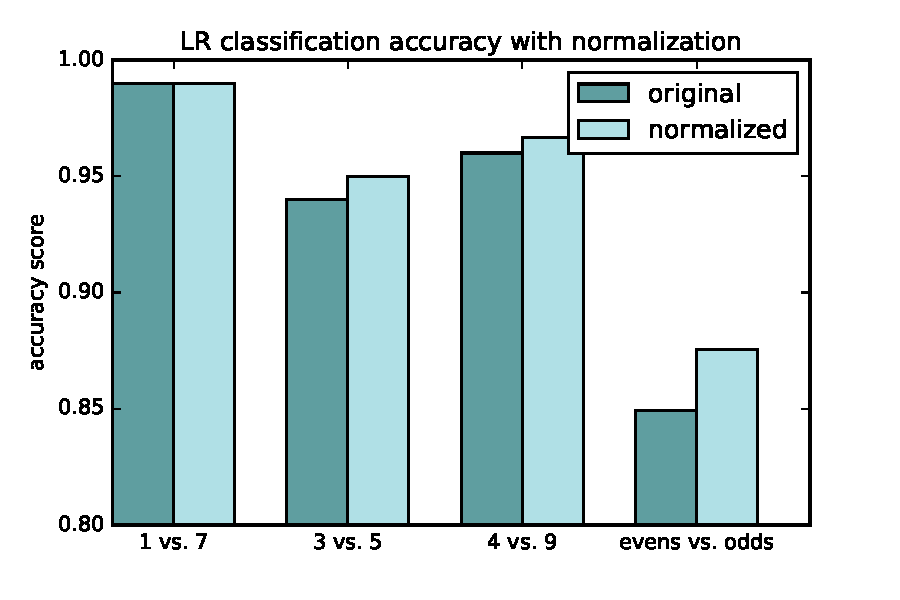
\includegraphics[width=3in]{img/4-1-normalization.pdf}
%	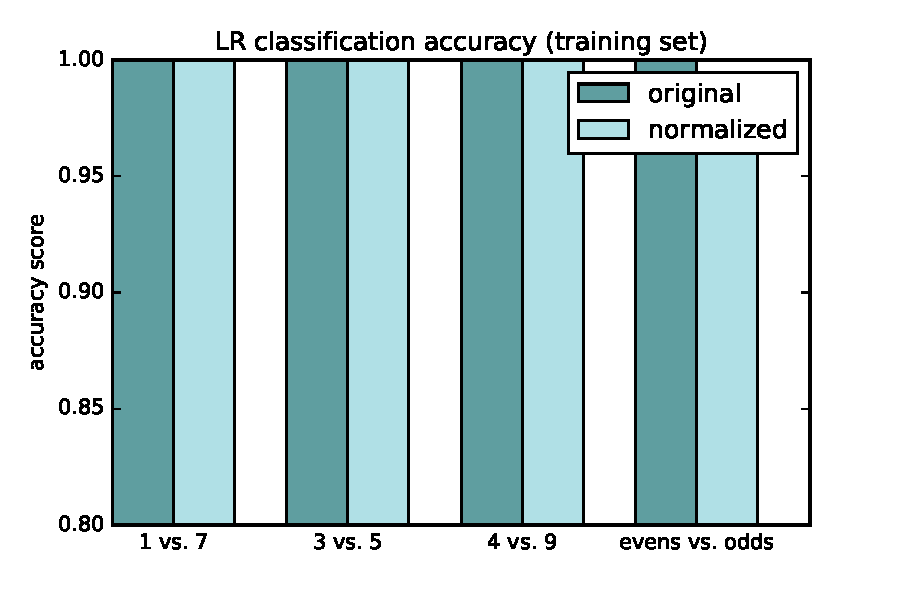
\includegraphics[width=3in]{img/4-1-normalization-train.pdf}
%   \caption{Effect of pixel feature normalization on classification accuracy, for logistic regression and SVM classifiers. Will fix later}
%   \label{fig:4-1-normalization}
%\end{figure*}
=======
We now run kernelized Pegasos (section~\ref{subsec:kernel-peg})
on the same four classification problems as above.
Our test set accuracies are below:  % TODO use actual numbers
\begin{center}    % TODO use actualnumbers
\begin{tabular}{|c|c|c|c|c|}
\hline
+ & - & $param_1$ & $param_2$ & Pegasos error \\\hline
1 & 7 &30 & 10 & 4/300 \\
3 & 5 &10 & 100 & 5/300\\
4 & 9 & 30 & 10 & 16/300\\
even & odd & - & - & - \\\hline
\end{tabular}
\end{center}

BLAH BLAH comparing accuracies % TODO

Finally, we consider the runtimes of
our quadratic-programming based approach and Pegasos.
For the 1/7 classification problem,
using Pegasos parameter $\lambda = 123123123$ with $12123$ epochs
% TODO change these numbers ^
(chosen because they produced comparably accurate results as our QP approach),
the training times of the two approaches increased as:
\begin{center}
    \begin{tabular}{|c|c|c|}\hline
        training set size & QP time (s) & Pegasos time (s) \\\hline
        200 & 18.1 & \\
        300 & 30.6 & \\
        400 & 46.3 & \\
        500 & 67.8 & \\\hline
    \end{tabular}
\end{center}
% TODO fill in for pegasos

% summarize and explain findings

>>>>>>> 63cea8e3329c87a999931d74990337ec6f9bd62b

\end{multicols}

\end{document}
